\subsection{Frontend Design}

I frontenden ønskes det at hele spillet foregår i et vindue. Det er derfor nødvendigt at programmet kan skifte mellem forskellige views uden at skulle åbne et nyt vindue, hver gang der skiftes. Løsningen til denne udfordring beskrives nærmere i implementerings afsnittet, nemlig \autoref{sec:Frontend Implementering}.
Spillet vil bestå af en række af vinduer, som giver spilleren den nødvændige information for at de kan spille spillet (så som at logge ind, gemme og hente spil, samt spille spillet).\\
Inden arbejdet på Frontend arkitekturen begyndte, er der blevet lavet en teknologiundersøgelse \autoref{sec:unity-.net}, om hvilket udviklingsværktøj Frontenden og derigennem spillet skulle udvikles i. Baseret på denne teknologiundersøgelse er der blevet valgt, at spillet vil blive udviklet i et .NET framework. Dette valg er blandt andet truffet da dette framework passer bedre med den opdeling af arbejde der er lavet i projektgruppen, altså opdelingen af Frontend og Backend. For andre grunde, se \textbf{(INDSÆT REFERENCE HER)}, hvor flere fordele og ulemper for både unity og .NET frameworket er sat op.\\
Her følger en række af mockups\footnote{Lavet i Unity} af nogle af spillets views.

\subsubsection{Room}

Room view (\autoref{fig:Design-FE-mockup-room}) er det primære spil-vindue. Her præsenteres spilleren for en beskrivelse af det rum de er i, samt hvilke elementer i rummet de kan interagere med. Der vises også et kort over banen. Kortet Viser kun de rum spilleren allerede har været i, mens resten holdes skjult. Når brugeren så besøger et nyt rum, kan dette ses selvom spilleren forlader rummet. Dette lader spilleren udforske og oplåse hele kortet.\\
En række knapper nederst i højre hjørne på skærmen giver spilleren mulighed for at interagere med spillet. Fire knapper ("Go {North/West/South/East}") lader spilleren gå fra et rum til et andet. Ikke alle rum har forbingelse til alle sider, så det er f.eks. ikke altid muligt at trykke på "Go North". Kortet og rum beskrivelsen fortæller hvilken vej det er muligt at bevæge sig i.\\
Udover de fire retningsknapper er der et antal andre knapper. Disse bruges til at gemme spillet, gå til menuer, samt interagere med elementerne i rummet. Det specifikke antal og deres funktion er afhængig af den præcise implementering.

\begin{figure}[H]
\centering
\includegraphics[width = \textwidth]{02-Body/Images/RoomMockup.PNG}
\caption{Et mockup af det primære spil vindue. Tekst øverst i venstre side af skærmen giver en beskrivelse af det rum spilleren er i, samt en liste af elementer i rummet som spilleren kan interagere med. Øverst til højre vises et billede af banen. Spilleren interagerer med spillet via knapper nederst i højre hjørne. Knapperne "Go {North/West/South/East}" fører spilleren ind i et andet rum, mens de resterende knapper (markeret "Button") bruges til andre funktionaliterer i spillet.}
\label{fig:Design-FE-mockup-room}
\end{figure}

\subsubsection{Combat}

Combat vinduet er baseret på room vinduet. Strukturen er den samme: der er et kort øverst til højre, en beskrivelse øverst til venstre og knapper neders til højre. Nederst til venstre er der information om hvordan kampen går,  i stedet for en liste af elementer i rummet.\\
Knapperne består af nogle "menu" knapper, som lader dig gå til spil menuer, samt en 'Fight' knap og en 'Flee' knap. 'Fight' knappen lader spilleren kæmpe mod fjenden, mens 'Flee' knappen lader spilleren flygte fra kampen og tilbage til rummet som spilleren kom fra.


\begin{figure}[H]
\centering
\includegraphics[width = \textwidth]{02-Body/Images/CombatMockup.PNG}
\caption{Combat view. Spilleren præsenteres for en fjende, og får information om hvordan kampen mod fjenden går. Der er knapper til at kæmpe og flygte, samt gå til menuer. øverst til højre er kortet over banen, ligesom i Room vinduet \autoref{fig:Design-FE-mockup-room}.}
\label{fig:Design-FE-mockup-combat}
\end{figure}


\subsubsection{Login}

Når spillet startes bedes spilleren prompte at logge ind på deres profil. Dette sker i login vinduet. Spilleren kan indtaste sit brugernavn og kodeord i de to tekstfelter 'Username' og 'Password'. Knappen login fører dem videre til spillet, hvis det indtastede login er korrekt.\\
Knappen create user fører spilleren til et vindue som ligner login vinduet, og som lader spilleren oprætte en ny bruger.\\
Exit lukker spillet.

\begin{figure}[H]
\centering
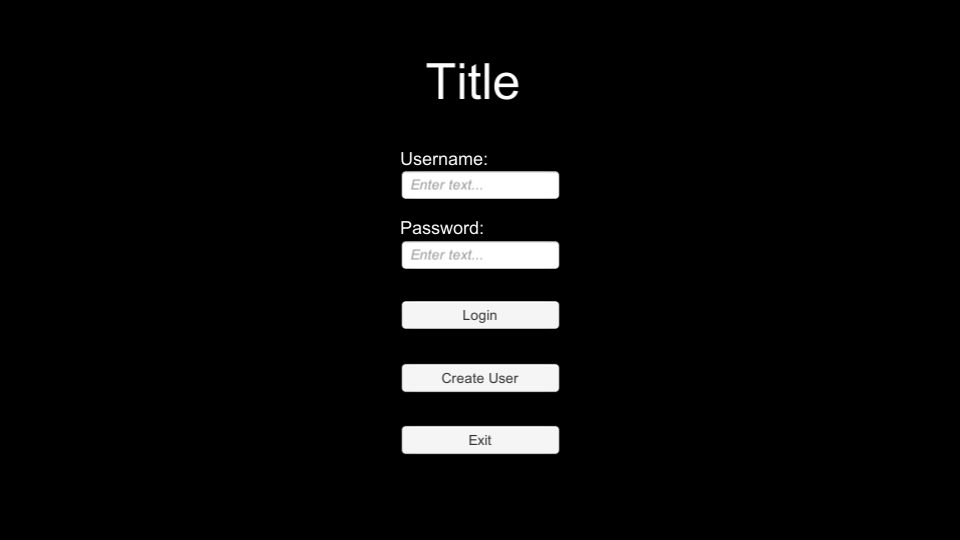
\includegraphics[width = \textwidth]{02-Body/Images/LoginMockup.PNG}
\caption{Login view. Bruger kan indtaste sit brugernavn og kodeord for at få adgang til spillet, eller trykke på create user for at komme til et vindue hvor man kan oprætte en ny bruger. Det er også muligt at forlade spillet igen.}
\label{fig:Design-FE-mockup-login}
\end{figure}

\subsubsection{Settings}
Settings viduet tillader at spilleren kan ændre indstillinger for spillet, og kan tilgås fra hovedmenuen, samt fra selve spillet.\\
Det er her muligt at ændre f.eks. skærmopløsning og lydstyrke. Det er muligt at gemme de indstillinger som er valgt, forlade menuen uden at gemme de valgte indstillinger, samt gendanne standard indstillingerne for spillet. 

\begin{figure}[H]
\centering
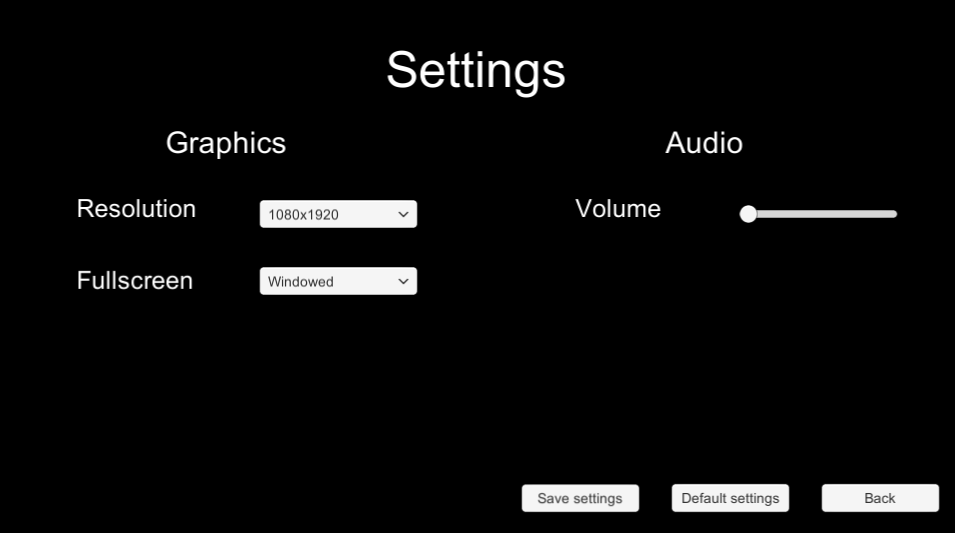
\includegraphics[width = \textwidth]{02-Body/Images/settingsMockup.PNG}
\caption{Settings view. Tillader at man kan ændre indstillinger for spillet, så som skærmopløsning og lydstyrke. Det er muligt at gemme indstillingerne, forlade skærmen uden at gemme indstillingerne, samt sætte spillet tilbage til standard indstilinger.}
\label{fig:Design-FE-mockup-settings}
\end{figure}

\newpage
